% Quiz 02 --- answer key. Instructor copy. Do not hand out.
% Compile with: xelatex -interaction=nonstopmode solutions.tex   (run twice)
\documentclass[a4paper, 12pt]{extarticle}
% Shared preamble for Quiz 02 (quiz02.tex and solutions.tex).
% Compile with: xelatex -interaction=nonstopmode <file>.tex   (run twice)
%
% Same house look as the pen-and-paper sheets in
% lecture-note/*/pen-and-paper/: Charter, A4, generous leading, room to draw.

\usepackage[top=0.7in, bottom=0.6in, left=0.8in, right=0.8in]{geometry}
\usepackage{amsmath}
\usepackage{amssymb}
\usepackage{array}
\usepackage{graphicx}
\usepackage[hidelinks]{hyperref}
\usepackage{tcolorbox}
\usepackage{enumitem}
\usepackage{etoolbox}
\usepackage{tikz}
\usepackage{fontspec}
\usetikzlibrary{calc,positioning,arrows.meta}
\definecolor{pltblue}{HTML}{1F77B4}
\definecolor{rulegrey}{HTML}{6A6D75}

% Body face. Charter, and the four ways to get it. XCharter *is* Charter and
% ships with a full TeX Live, so it is asked for first and by file: a CI runner
% answers yes to \IfFontExistsTF{Charter}, then cannot typeset it.
\IfFontExistsTF{XCharter-Roman.otf}{
  \setmainfont{XCharter}[
    Extension      = .otf,
    UprightFont    = *-Roman,
    BoldFont       = *-Bold,
    ItalicFont     = *-Italic,
    BoldItalicFont = *-BoldItalic]
}{
  \IfFontExistsTF{Charter}{\setmainfont{Charter}}{
    \IfFontExistsTF{Iowan Old Style}{\setmainfont{Iowan Old Style}}{
      \IfFontExistsTF{Georgia}{\setmainfont{Georgia}}{}}}}

\setlength{\parindent}{0pt}
\setlength{\parskip}{0.4em}
\setlength{\emergencystretch}{1.2em}
\raggedbottom
\pagestyle{empty}

% ---------------------------------------------------------------------------
% The submission link.
%
% Both the QR square and the printed address are the course's own short link,
% not the form's: paper outlives any one form. Caddy on the course droplet
% points go.skojaku.com/ans-quiz02 at the current Google Form
% (/etc/caddy/Caddyfile, block go.skojaku.com). Swapping the form is a line on
% the server, not a reprint.
%
% If the link ever changes, rebuild the square with
%
%   uvx --from segno segno --output=quiz02-form-qr.png --scale=20 --border=1 \
%       --error=m "<the url>"
%
% PNG rather than PDF for the square: segno's PDF is too spare for xdvipdfmx to
% include, and a QR is squares, so 700px across a 3cm box is already sharper
% than the printer.
% ---------------------------------------------------------------------------
\newcommand{\formlink}{https://go.skojaku.com/ans-quiz02}
\newcommand{\formshort}{\href{\formlink}{\texttt{go.skojaku.com/ans-quiz02}}}

% Quiz header. #1 = title, #2 = the line under it, #3 = term.
\newcommand{\quizhead}[3]{%
  {\footnotesize\textsc{Advanced Network Science} \hfill \textsc{#3}}\par
  \vspace{-0.2em}\rule{\textwidth}{1pt}\par
  \vspace{0.3em}
  {\LARGE\bfseries #1}\par
  \vspace{0.1em}
  {\small #2}\par
  \vspace{0.7em}
  {\small Name \underline{\hspace{6cm}} \hfill Date \underline{\hspace{3.2cm}}}\par
  \vspace{0.7em}}

% A question heading with its point value.
\newcommand{\question}[3]{%
  \vspace{0.5em}
  {\large\bfseries Question #1 \quad\normalsize\mdseries (#2 points)}\par
  \vspace{-0.3em}{\color{rulegrey}\rule{\textwidth}{0.6pt}}\par
  \vspace{0.1em}
  {\bfseries #3}\par
  \vspace{0.2em}}

% An empty box to draw or write in. #1 = height, #2 = caption under the rule.
\newcommand{\drawbox}[2]{%
  \begin{tcolorbox}[colback=white, colframe=rulegrey, boxrule=0.5pt,
                    sharp corners, height=#1, valign=top,
                    boxsep=2pt, left=4pt, right=4pt, top=3pt, bottom=3pt]
  {\footnotesize\color{rulegrey} #2}
  \end{tcolorbox}}

% Ruled writing lines, #1 of them.
\newcommand{\writelines}[1]{%
  \vspace{0.3em}
  \foreach \i in {1,...,#1}{%
    {\color{rulegrey}\rule{\textwidth}{0.4pt}}\par\vspace{1.5em}}}


\tikzset{
  gnode/.style={circle, draw=pltblue, fill=pltblue!12, line width=0.9pt,
                minimum size=7mm, inner sep=0pt, font=\small\bfseries},
  gedge/.style={line width=0.9pt, draw=rulegrey},
  gtri/.style={line width=2.2pt, draw=pltblue!55}
}

% A grading note, set apart from the answer itself.
\newenvironment{grading}
  {\begin{tcolorbox}[colback=pltblue!4, colframe=pltblue!35, boxrule=0.5pt,
                     sharp corners, boxsep=2pt, left=6pt, right=6pt,
                     top=4pt, bottom=4pt]\small\textbf{Marking.}\ }
  {\end{tcolorbox}}

\begin{document}

{\footnotesize\textsc{Advanced Network Science} \hfill \textsc{Fall 2026}}\par
\vspace{-0.2em}\rule{\textwidth}{1pt}\par
\vspace{0.3em}
{\LARGE\bfseries Quiz 2 \; --- \; Answer key}\par
\vspace{0.1em}
{\small Instructor copy. Answers below are models, not the only correct ones.}\par
\vspace{0.8em}

% ---------------------------------------------------------------------------
\question{1}{6}{Measure this network.}

The network has 6 nodes and 7 edges. Degrees:
$\deg A = 5$, $\deg B = \deg C = \deg E = \deg F = 2$, $\deg D = 1$.
The two triangles are drawn thick.

\begin{center}
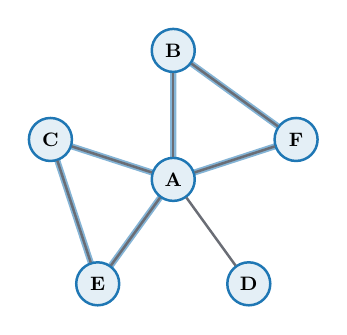
\begin{tikzpicture}[scale=0.78, every node/.style={transform shape}]
  \draw[gtri] (0,0) -- (0,2.1) -- (2.0,0.65) -- cycle;
  \draw[gtri] (0,0) -- (-2.0,0.65) -- (-1.23,-1.70) -- cycle;
  \node[gnode] (A) at ( 0.00,  0.00) {A};
  \node[gnode] (B) at ( 0.00,  2.10) {B};
  \node[gnode] (F) at ( 2.00,  0.65) {F};
  \node[gnode] (D) at ( 1.23, -1.70) {D};
  \node[gnode] (E) at (-1.23, -1.70) {E};
  \node[gnode] (C) at (-2.00,  0.65) {C};
  \draw[gedge] (A) -- (B); \draw[gedge] (A) -- (C); \draw[gedge] (A) -- (D);
  \draw[gedge] (A) -- (E); \draw[gedge] (A) -- (F);
  \draw[gedge] (B) -- (F); \draw[gedge] (C) -- (E);
\end{tikzpicture}
\end{center}

\textbf{(a) [3 pts]} \emph{Triangles:} $ABF$ and $ACE$, so \textbf{2}.

\emph{Connected triples:} a node contributes $\binom{\deg}{2}$.
\[
  \underbrace{\tbinom{5}{2}}_{A} + \underbrace{\tbinom{2}{2}}_{B}
  + \underbrace{\tbinom{2}{2}}_{C} + \underbrace{\tbinom{1}{2}}_{D}
  + \underbrace{\tbinom{2}{2}}_{E} + \underbrace{\tbinom{2}{2}}_{F}
  = 10 + 1 + 1 + 0 + 1 + 1 = \mathbf{14}.
\]
\[
  C \;=\; \frac{3 \times 2}{14} \;=\; \frac{3}{7} \;\approx\; \mathbf{0.43}.
\]

\begin{grading}
One point each for the triangle count, the triple count, and the value.
Watch for two things. \textbf{The average \emph{local} clustering coefficient
is a different number} --- $\frac{1}{6}(0.2 + 1 + 1 + 0 + 1 + 1) = 0.7$ --- and
the sheet asked for the global one; a student who computes $0.7$ correctly
keeps at most 1 point, for the per-node work. \textbf{Dropping the factor $3$}
gives $1/7 \approx 0.14$: keep both counting points, lose the third.
\end{grading}

\textbf{(b) [3 pts]} There are $\binom{6}{2} = 15$ pairs.

\emph{Distance 1} --- one pair per edge, so \textbf{7}: $AB$, $AC$, $AD$,
$AE$, $AF$, $BF$, $CE$.

\emph{Distance 2} --- the remaining \textbf{8} pairs. Every one of them is two
non-neighbours among $\{B,C,D,E,F\}$, and each is joined through $A$: $BC$,
$BD$, $BE$, $CD$, $CF$, $DE$, $DF$, $EF$. Nothing is further, because $A$ is
adjacent to everything.
\[
  \langle \ell \rangle \;=\; \frac{7 \times 1 + 8 \times 2}{15}
  \;=\; \frac{23}{15} \;\approx\; \mathbf{1.53}.
\]

\begin{grading}
One point for the split ($7$ at distance 1, $8$ at distance 2), one for the sum
$23$, one for $23/15$. Counting \emph{ordered} pairs gives $46/30$, the same
number --- full marks. Dividing by $36$ or $21$ (self-pairs included) loses the
third point only.
\end{grading}

\newpage
% ---------------------------------------------------------------------------
\question{2}{4}{A tempting index.}

For the network above, $S = \dfrac{3/7}{23/15} = \dfrac{45}{161} \approx 0.28$.

\textbf{(a) [3 pts]} \textbf{$S$ has no baseline, and its two halves do not
live on the same scale.} ``Small world'' is a \emph{comparative} claim: paths
as short as in a random network of the same size and density, while clustering
is far higher than that random network's. $S$ compares nothing --- it divides a
bounded quantity by an unbounded one:

\begin{itemize}[leftmargin=1.4em, itemsep=0.15em, topsep=0.2em]
\item $C \in [0,1]$ always. $\langle \ell \rangle$ grows with the number of
      nodes, roughly like $\log n / \log \langle k \rangle$. So $S$ falls as a
      network gets bigger \emph{whatever its structure}, and two networks of
      different sizes cannot be compared with it at all.
\item The maximum of $S$ is the complete graph: $C = 1$, $\langle\ell\rangle
      = 1$, $S = 1$. Nobody calls a clique a small world --- it has no long
      distances to shorten.
\end{itemize}

\emph{A concrete inversion.} A $1000$-node Watts--Strogatz ring at a small
rewiring probability is the textbook small world: $C \approx 0.5$,
$\langle\ell\rangle \approx 5$, so $S \approx 0.1$. The six-node network on the
front of this sheet --- a star with two extra edges, and no small-world
character whatever --- scores $S \approx 0.28$. $S$ ranks it nearly three times
the more ``small-world'' of the two.

\emph{Two further breakages, either of which earns the point on its own:} any
triangle-free network has $C = 0$ and therefore $S = 0$, however short its
paths; and $\langle\ell\rangle$ is undefined (or infinite) the moment the
network is disconnected, so $S$ cannot be computed for most real data.

\begin{grading}
Three points, one each:
\textbf{(i)} naming the missing baseline --- that small-worldness has to be
measured \emph{against} something, normally a randomized network with the same
size and degrees.
\textbf{(ii)} an argument for \emph{why} the raw ratio cannot work: the size
dependence above, or that a bounded numerator over an unbounded denominator is
not a meaningful quantity. ``It is not normalized'' with no reason is not the
point.
\textbf{(iii)} a counterexample that actually holds. \emph{Check it} --- a
student who asserts an inversion without numbers, or whose numbers do not
invert, earns nothing for this third point. The clique, the two-network
comparison, the $C = 0$ tree, and the disconnected network are all full credit.

A student who instead attacks $S$ for being \emph{unitless but not scale-free},
or for mixing a per-triple ratio with a per-pair mean, has named the same
defect in other words --- give (i) and (ii).
\end{grading}

\textbf{(b) [1 pt]} Normalize each half against a randomized network with the
same number of nodes and the same degree sequence (a configuration-model
rewiring), and average over several draws:
\[
  \sigma \;=\; \frac{C / C_{\text{rand}}}{\langle\ell\rangle /
  \langle\ell\rangle_{\text{rand}}}, \qquad \sigma \gg 1
  \;\Longrightarrow\; \text{small world.}
\]
It compares the network against a version of \emph{itself} with the same size
and degrees but the edges shuffled, so ``high clustering'' and ``short paths''
both mean high and short \emph{relative to chance}.

\begin{grading}
The one point needs \textbf{both}: a definition that divides through by a
reference, \emph{and} a sentence saying what the reference is. $\sigma$ is the
model answer; Telesford's
$\omega = \langle\ell\rangle_{\text{rand}}/\langle\ell\rangle - C/C_{\text{latt}}$
is equally correct, and so is any home-made index that compares against a
randomized null. ``Divide by a random graph'' with no statement of which random
graph earns nothing --- the same-degree constraint is the whole content.
\end{grading}

\end{document}
